% Autor: Simon May
% Datum: 2017-10-05
% Diese Datei bietet ein minimalistisches Grundgerüst für ein LaTeX-Dokument,
% z.B. für die Bearbeitung der Aufgaben.
\documentclass[
	% Papierformat
	a4paper,
	% Schriftgröße (beliebige Größen mit „fontsize=Xpt“)
	12pt,
	% Schreibt die Papiergröße korrekt ins Ausgabedokument
	pagesize,
	% Sprache für z.B. Babel
	ngerman
]{scrartcl}

% Achtung: Die Reihenfolge der Pakete kann (leider) wichtig sein!
% Insbesondere sollten (so wie hier) babel, fontenc und inputenc (in dieser
% Reihenfolge) als Erstes und hyperref und cleveref (Reihenfolge auch hier
% beachten) als Letztes geladen werden!

% Silbentrennung etc.; Sprache wird durch Option bei \documentclass festgelegt
\usepackage{babel}
% Verwendung der Zeichentabelle T1 (Sonderzeichen etc.)
\usepackage[T1]{fontenc}
% Legt die Zeichenkodierung der Eingabedatei fest, z.B. UTF-8
\usepackage[utf8]{inputenc}
% Schriftart
\usepackage{lmodern}
% Zusätzliche Sonderzeichen
\usepackage{textcomp}

% Mathepaket (intlimits: Grenzen über/unter Integralzeichen)
\usepackage[intlimits]{amsmath}
% Ermöglicht die Nutzung von \SI{Zahl}{Einheit} u.a.
\usepackage{siunitx}
% Zum flexiblen Einbinden von Grafiken (\includegraphics)
\usepackage{graphicx}
% Abbildungen im Fließtext
\usepackage{wrapfig}
% Abbildungen nebeneinander (subfigure, subtable)
\usepackage{subcaption}
% Funktionen für Anführungszeichen
\usepackage{csquotes}
% Zitieren, Bibliographie
\usepackage{biblatex}

% Verlinkt Textstellen im PDF-Dokument
\usepackage[unicode]{hyperref}
% "Schlaue" Referenzen (nach hyperref laden!)
\usepackage{cleveref}

% siunitx: Deutsche Ausgabe, Messfehler getrennt mit ± ausgeben
\sisetup{
	locale=DE,
	separate-uncertainty
}

\begin{document}
\begin{titlepage}
	\centering
	{\scshape\LARGE Versuchsbericht zu \par}
	\vspace{1cm}
	{\scshape\huge O4 - Magneto-Optischer-Kerr-Effekt \par}
	\vspace{2.5cm}
	{\LARGE Gruppe 6 Mo\par}
	\vspace{0.5cm}
	{\large Nils Kulawiak (E-Mail: n\_kula01@wwu.de) \par}
	{\large Oliver Brune (E-Mail: o\_brun02@wwu.de) \par}
	\vfill
	durchgeführt am 11.06.2018\par
	
	\vfill
	betreut von Christoph Angrick
	{\large \today\par}
\end{titlepage}

\tableofcontents
		
\newpage


\section{Methoden und Durchführung}
Zuerst mussten alle verwendeten Proben um einen bestimmten Grad verformt werden. Dafür wurden sie mit einer Walze dünner gewalzt. Um einen bestimmten Verformungsgrad zu erreichen, wurde zuerst mit \cref{eq:ver} die benötigte Dicke der Probe berechnet. Die Probe wurde anschließend auf die berechnete Dicke gewalzt.

\begin{equation}
V = \frac{d_0-d}{d_0} \cdot 100
\label{eq:ver}
\end{equation}

Anschließend wurden die Proben in verschiedene Öfen gegeben. Einerseits wurden sieben Proben, die alle auf einen Verformungsgrad von $80\%$ verformt wurden, auf sieben Öfen mit verschiedenen Temperaturen verteilt, in denen sie jeweils fünf Minuten erhitzt wurden. Eine Probe wurde nicht erhitzt, sondern bei Raumtemperatur gelassen. Andererseits wurden acht Proben mit verschiedenen Verformungsgraden in einem Ofen mit $550\%$ für eine Stunde erhitzt. Alle Proben wurden nach der Zeit im Ofen in kaltem Wasser schnell auf Raumtemperatur abgekühlt, um die Ergebnisse durch einen langsamen Abkühlprozess nicht zu verfälschen. Die beiden Probenpakete wurden anschließend mit unterschiedlichen Verfahren weiter untersucht.

Bei den Proben mit gleichem Verformungsgrad, aber unterschiedlicher Heiztemperatur, wurde im weiteren die Vickers-Härte gemessen. Hierbei wird ein Diamant in Form einer Pyramide mit fester Kraft für fünf Sekunden in die Probe gedrückt. Die Vickers-Härte wird nun aus der Eindringtiefe der Pyramide und der Kraft, mit der auf die Probe gedrückt wird, berechnet. Die Eindringtiefe wird aus der Breite des Abdrucks der Pyramide bestimmt. Diese Rechnung führt der verwendete Vickers-Härteprüfer automatisch aus. Da die Härte eines Stoffs bei starker Verformung steigt, ist die Vickers Härte in diesem Versuch ein Maß dafür, wie stark die Kristallbaufehler der Proben nach der Zeit im Ofen ausgeheilt sind. Eine höhere Vickers-Härte bedeutet daher starke Verformung, also viele Kristallbaufehler, eine niedrige Vickers-Härte steht für schwache Verformung, also eine stark ausgeheilte Probe. Für jede Probe wurden drei Werte aufgenommen.

\section{Auswertung}

In \cref{vickers} wurde die Vickers-Härte gegen die Temperatur aufgetragen. Von Raumtemperatur bis etwa $\SI{140}{\degreeCelsius}$ ist die Vickers-Härte nahezu konstant bei $44-45$HV. Zwischen $\SI{190}{\degreeCelsius}$ und $\SI{350}{\degreeCelsius}$ sinkt die Härte, bis sie einen Wert von $22$ HV erreicht. Für höhere Temperaturen bleibt die Vickers-Härte konstant auf diesem Wert.

\begin{figure}[h]
	\centering
	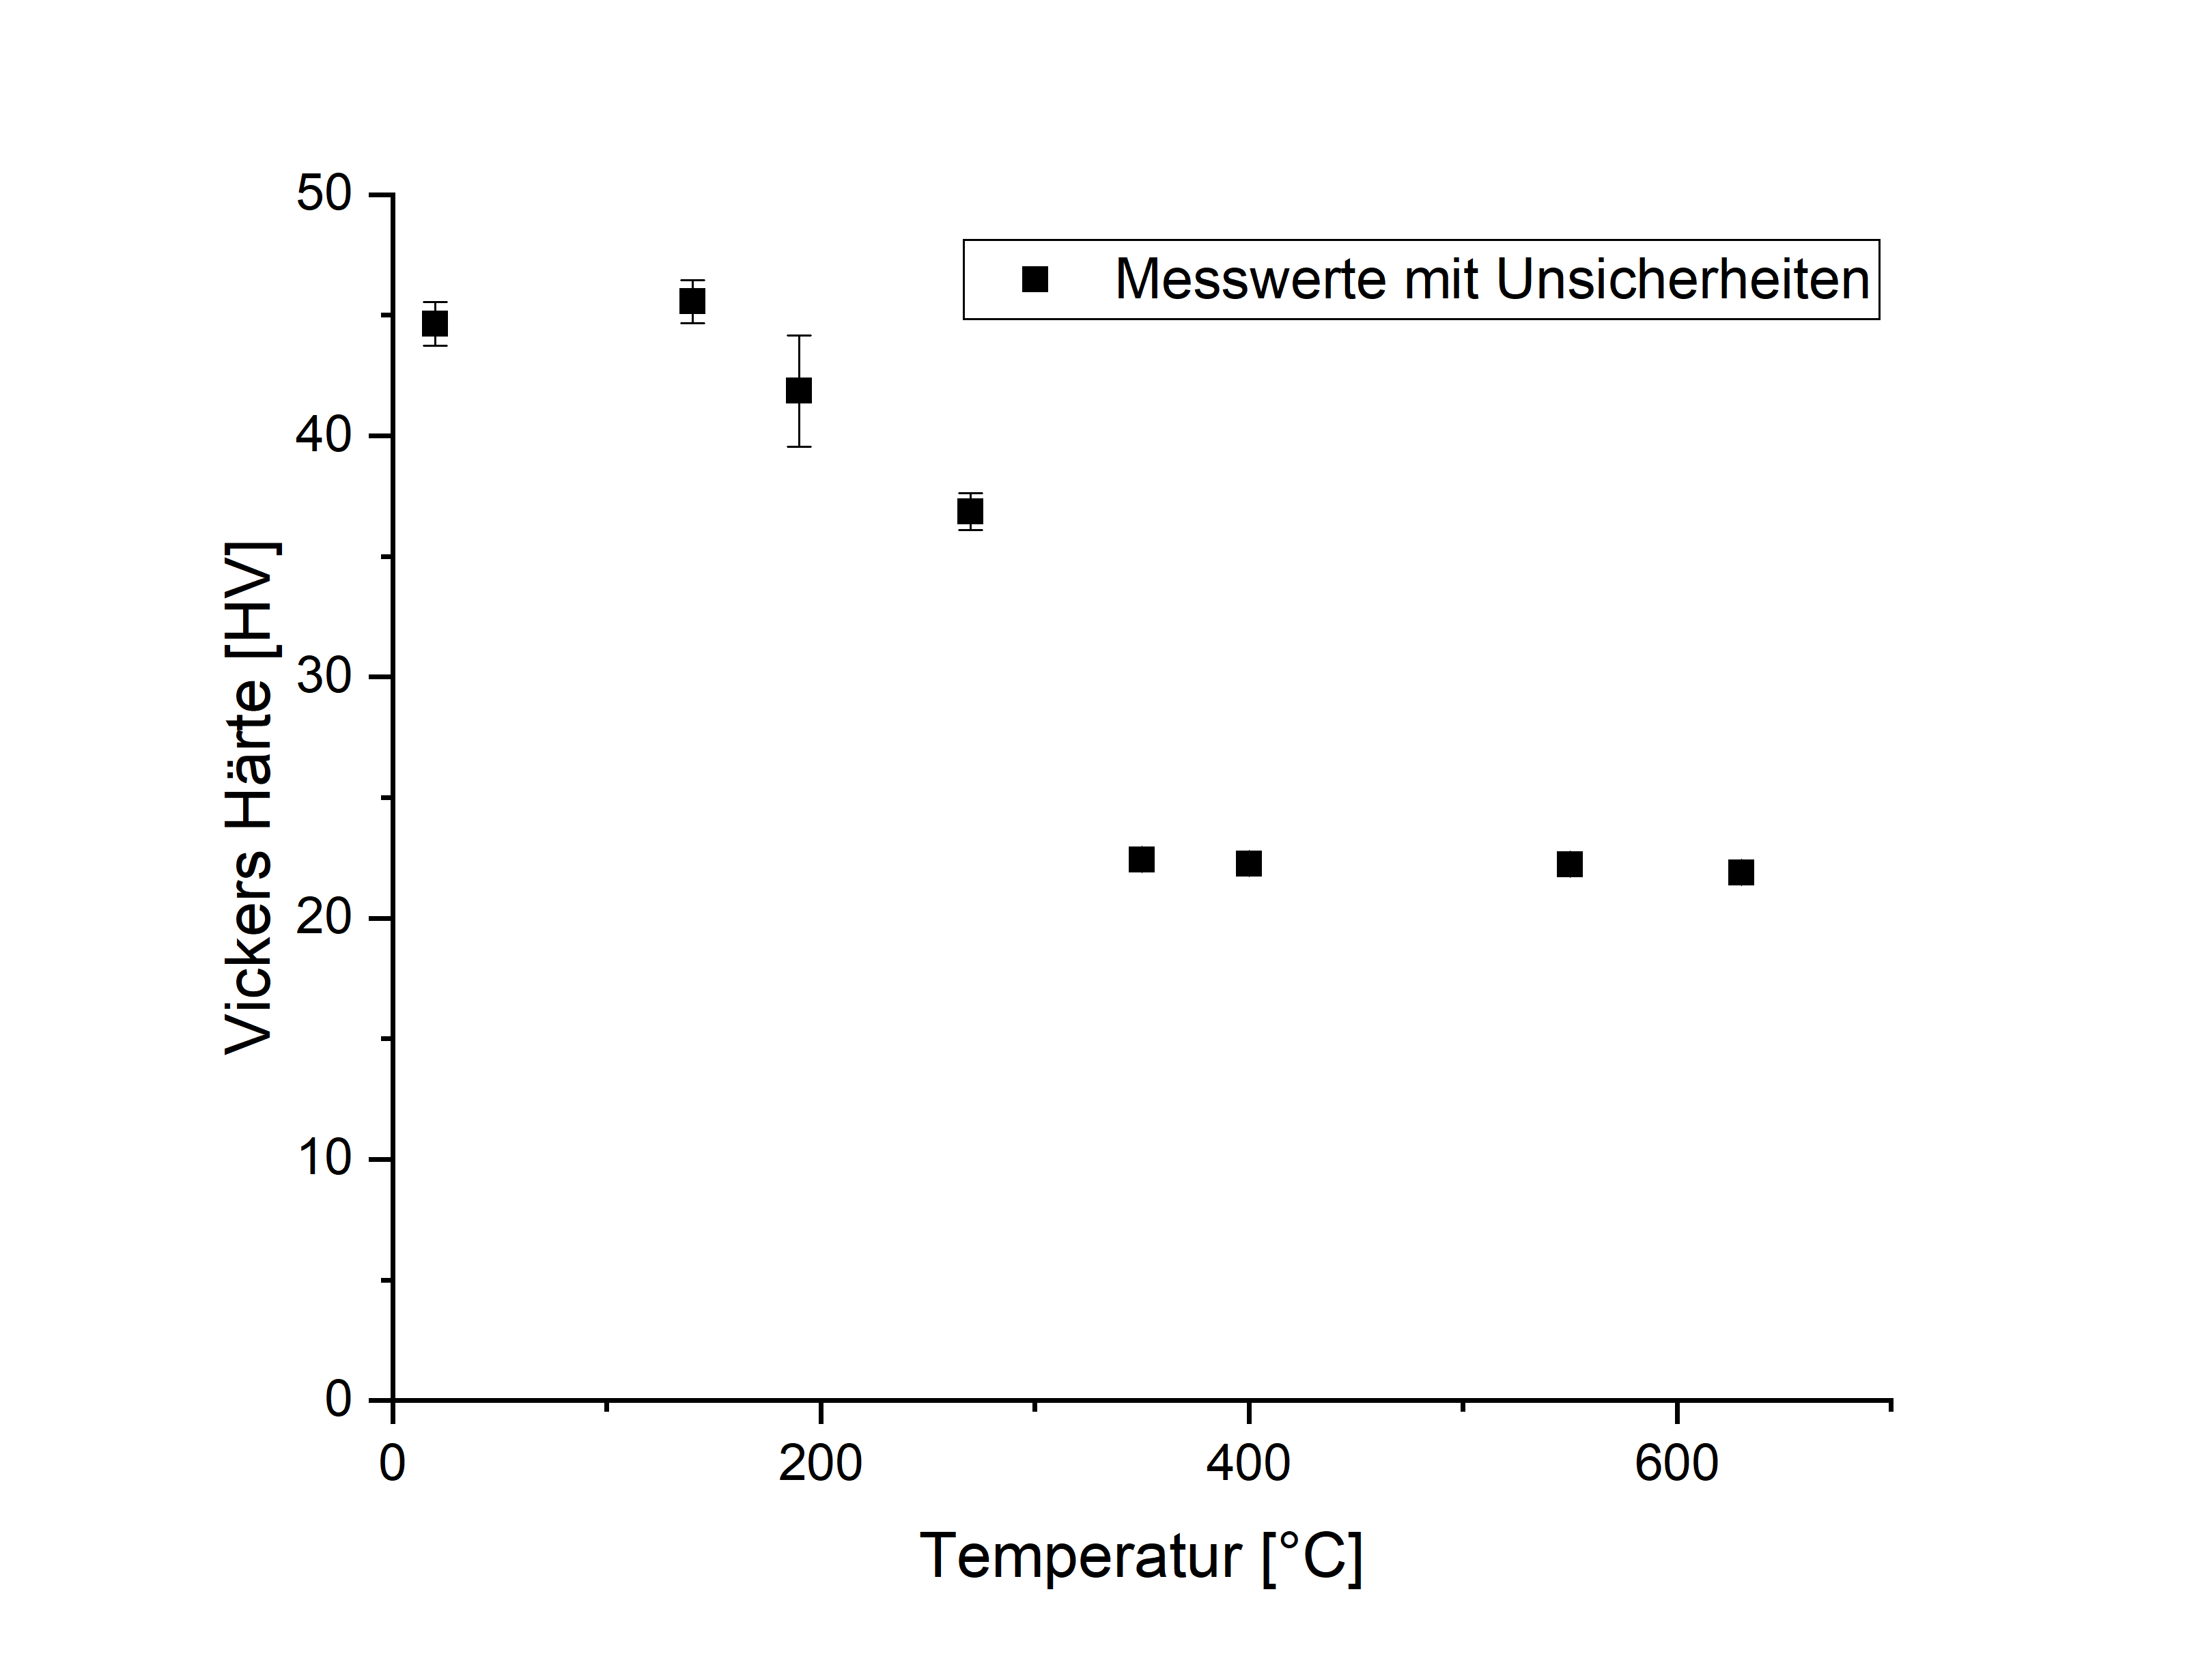
\includegraphics[scale=0.6]{vickers.png}
	\caption{Die Vickers-Härte aufgetragen gegen die Temperatur, bei der die Probe vorher für fünf Minuten im Ofen erhitzt wurde.}
	\label{vickers}
\end{figure}

Die Unsicherheit ergibt sich aus der Standardabweichung um den Mittelwert, der aus den drei Messwerten pro Probe berechnet wird. Sie ist nur für die Probe bei $\SI{190}{\degreeCelsius}$ mit $\pm2,31$ etwas größer, ansonsten ist sie vernachlässigbar klein.

\begin{figure}[h]
	\centering
	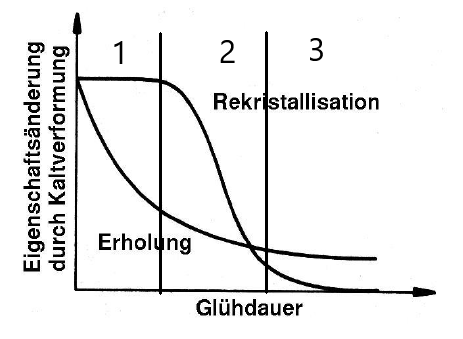
\includegraphics[scale=1]{grafik1.png}
	\caption{Zeitlicher Ablauf der Erholung und Rekristallisation (schematisch)}
	\label{grafik}
\end{figure}

Bei der Ausheilung von Kristallbaufehlern spielen zwei Prozesse eine Rolle: Erholung und Rekristallisation. Die Rekristallisation ist stark von der Temperatur abhängig. Die Zeit, die ein Kristall zur Rekristallisation benötigt, sinkt exponentiell bei höherer Temperatur. Eine Rolle spielt außerdem die unterschiedliche Geschwindigkeit, mit der beide Prozesse ablaufen. Die Kinetik beider Prozesse ist in \cref{grafik} dargestellt, außerdem sind drei Phasen der Rekristallisation eingezeichnet. Die Erholungsgeschwindigkeit ist zu Beginn am größten, sinkt aber über längere Zeit immer weiter ab.Bei der Rekristallisation dagegen müssen sich zuerst neue Körner bilden. In diesem Zeitraum bleibt die Verformung konstant (Phase 1). Nach einiger Zeit fangen die Körner stärker an zu wachsen, hier werden sehr schnell viele Kristallbaufehler berichtigt (Phase 2). Wenn die Körner so groß geworden sind, dass sich die Korngrenzen berühren, endet der Prozess, die Verformung bleibt konstant (Phase 3). Über diese beiden Zusammenhänge lässt sich der Verlauf der Messwerte in \cref{vickers} erklären.

Bei den ersten beiden Temperaturen ist die Rekristallisationszeit noch sehr groß, die Keime bilden sich so langsam, dass sich die Rekristallisation nach den fünf Minuten im Ofen noch in Phase 1 befindet. Die Proben von $\SI{190}{\degreeCelsius}$ bis $\SI{350}{\degreeCelsius}$ befinden sich nach der Erhitzung in Phase 2, es haben sich bereits größere Körner gebildet, diese sind allerdings noch nicht ausgewachsen. Die restlichen Proben sind nach fünf Minuten im Ofen bereits vollständig rekristallisiert, sie befinden sich in Phase 3. Die Rekristallisationszeit ist hier kleiner als fünf Minuten.

Die Vickers-Härte, und damit auch die Ausheilung der Proben, ist in diesem Versuch unabhängig von der Erholung und lässt sich vollständig durch Rekristallisation erklären. Das liegt daran, dass die Erholung am Anfang stark ist und mit der Zeit schwächer wird und nicht so stark von der Temperatur abhängt wie die Rekristallisation, sondern auch bei Raumtemperatur stattfindet. Da zwischen der Verformung der Proben und der Messung der Vickers-Härte mehrere Stunden lagen, konnten sich die Proben in dieser Zeit bereits sehr stark erholen. Da die Erholung nach längerer Zeit sowieso kaum noch Auswirkung auf die Ausheilung hat, spielt sie für den Verlauf der Messwerte in \cref{vickers} keine Rolle.
\end{document}